\chapter{Introduction}

\section{Background and motivation}

\subsection{Procedural generation in games}

The industry of computer games is a big and serious business, even bigger than those of film and music.\cite{web-gamebigindustry} The global market size was estimated to be 83 billion USD in 2014, and is expected to surpass 100 billion by 2018.\cite{web-gamesmarket2018} Not only the revenue is growing, producing a game is also becoming increasingly expensive. \gameref{gta5} (2013), for example, has the production cost of 265 million USD, including both development and marketing.\cite{web-gta5}

Much of the development cost of a video game can be attributed to \textit{content generation}, estimated from anecdotal evidences to be in the range of 30\%--40\% of total budget.\cite{hendrikx2013procedural} The generated content covers everything from elementary bits and pieces -- textures, sound, vegetation, etc. -- to more sophisticated ones such as maps, stories, puzzle elements, and even the rules of the game themselves. It usually takes large teams of highly-skilled human creators to produce game content. \gameref{starwars-tor} (2011), whose development cost alone was estimated to be almost 200 million USD, was developed by teams of more than 800 people across four continents, for 6 years.\cite{web-oldrepublic} For \gameref{destiny} (2014) it took around 500 people to manually create most of the content.\cite{web-expensivedevelop}

With the amount of resources -- both time and money -- currently being spent to create content for modern games, it is tempting to try to do it automatically, rather than manually. \textbf{Procedural generation} is a technique that aims to accomplish this. Togelius et al.\cite{togelius2011procedural}\ defined procedural generation as `the creation of game content automatically using algorithms'\footnote{The actual definition is for the term \textbf{procedural content generation}, as opposed to \textbf{procedural generation}, which in some context is limited to only the process of generating content that does not affect gameplay \textit{significantly}. (See \url{http://pcg.wikidot.com/pcg-algorithm:procedural-generation}) However, in this work these two terms will be used interchangeably.}. Historically, the motivation for procedural generation was not always about cost reduction. Computer programs used to operate at extremely limited amount of memory. Procedural generation helps in this aspect by producing large amount of content dynamically at run-time, effectively packing a lot of information into very small amount of memory, comparing to static content. Moreover, since procedural-generated content is generated randomly, it increases variety, and thus replayability for the games. %citation?

Various types of game content have been created procedurally since the early days of video games. The roguelike genre and its relatives -- games such as \gameref{rogue} (1980), \gameref{angband} (1990), \gameref{diablo} (1996), or \gameref{dwarffortress} (2006) -- all feature adventures in procedural-generated dungeons. \gameref{spelunky} (2008) also uses procedural generation to create its dungeon, but in a vertical 2-D, platformer style. Maps in the strategy game series \gameref{civ} (1991) are also generated procedurally, and play a crucial role in the massive success of these games\cite{web-7usesofprocgen}. Another example of success application of procedural generation is \textit{SpeedTree}, a tool that generates vegetation procedurally. It has been used extensively in commercial games, and also in film industry -- starting from James Cameron's \textit{Avatar} in 2009.\cite{web-speedtree}

\begin{figure}
	\centering
	\includegraphics[width=.7\linewidth]{figures/Spelunky.png}
	\caption{A procedurally-generated vertical level in \textit{Spelunky}.}
\end{figure}

\subsection{Tactical role-playing game}

Tactical role-playing game (TRPG) is a sub-genre of role-playing game (RPG)\cite{stenstrom2013understanding}, but also sometimes classified as a type of strategy wargame, incorporating elements from both genres. It is also known as \textit{strategy RPG}, or \textit{simulation RPG}.\cite{web-srpg} Classic examples of the genre include \gameref{fireemblem} (1990), \gameref{fft} (1997), and the \gameref{disgaea1} franchise (2003)\cite{web-playingroles}.

\begin{figure}
	\centering
	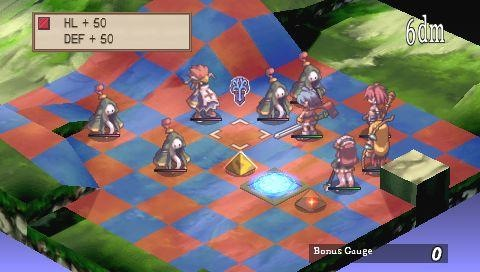
\includegraphics[width=.7\linewidth]{figures/disgaea_aod.jpg}
	\caption{A battle scene from the tactical RPG \textit{Disgaea: Afternoon of Darkness}.}
\end{figure}

Among the various sub-genres of RPG, tactical RPG could be characterised as the one with the strongest emphasis on combats, at the expense of world exploration.\cite{stenstrom2013understanding} The focus of a TRPG is on battle scenes, which take place on some sort of grids (usually square), where two players each take control of a party of units, moving them around and attacking or defending from the other party. The same description could also be used to describe strategy games, spanning from abstract strategy board games such as chess, checkers, or go, to the modern computer games in the genre of \textit{real-time strategy} (RTS), such as \gameref{warcraft} (1994), \gameref{cnc} (1995), or \gameref{starcraft} (1998). TRPG has so much in common with the strategy games, that it is sometimes called `mini-wargame', and grouped together with strategy games rather than RPG.\cite[92, 108]{moore2011basics} The key difference that distinguishes RPG from strategy, however, is that of \textit{perspectives}. In RPG, players are asked to identify with a character (or a party of characters), while in strategy games, characters are treated more like dispensable resources that are produced from some sort of factories.\cites[8]{barton2008dungeons}[455]{adams2010fundamentals} In this sense, TRPG definitely belongs to the RPG genre.

The complexity of a TRPG arises from the range and combination of moves and actions each unit can perform. In contrast to other types of RPG where battles are trending towards being real-time, TRPG retains the primary turn-based nature of traditional tabletop RPG.\cite[90]{moore2011basics} This allows players to plan and experiment with different options, favouring tactical skills over responsiveness.

\subsection{Game balance}

Balance is one of the most crucial part of any games. It is considered to be the most subtle part of game design; an art, rather than science.\cite{schell2008art} As TRPG focuses so heavily on the combats, one of the primary aspects that need to be in balance is the effect of each of the choices available to the players on the combat, which we collectively call the \textbf{battle system}. This includes things such as classes and races of the characters, strength and attacking range of weapons, effectiveness of armours against different types of attacks, etc.

Striking good balance is usually carried out by a long and tedious process of \textit{manual testing} and \textit{fine-tuning}. Automating the process would potentially lead to rewarding benefits. %some ref here would be nice
However, procedural generation tends to be used more on peripheral aspects of games; producing texture, sounds, vegetation, and maps, are some of the most common applications.\cite{hendrikx2013procedural} Battle systems, on the other hand, are central to the gameplay of TRPG, and has not been explored as much. This leads us to ask:

\begin{tcolorbox}
	How can procedural generation be used to create balanced battle systems for tactical role-playing games automatically?
\end{tcolorbox}

This is the main research question that this work will attempt to address.

\section{Objectives}

The aim of this work is to study the possibility of using procedural generation to generate battle systems in a balanced way. To achieve this, the following objectives are the primary ones that need to be met:

\begin{itemize}
	\item A \textbf{prototype TRPG}, as a playable game on its own. As our focus is solely on the battles, other aspects of typical TRPG such as character progression or storytelling can be ignored. To allow human players to play the game and observe the ensuing battles, a user interface for the game is required, though it does not have to be sophisticated -- a simple command line interface, for example, would suffice.
	
	\item The \textbf{battle mechanics} of the prototype must support these minimal aspects of typical TRPG gameplay:
	\begin{itemize}
		\item Battles are won by removing all the opponent's units.
		\item Characters possess a small set of basic attributes that builds up more complex ones.
		\item Standard action types are supported: physical melee attack, long range attack, magical attack, and healing.
	\end{itemize}

	\item An \textbf{AI player}. It is an essential part of the battle system evaluation process. The AI must be generic enough to play the game for any generated battle systems, in a reasonably competent manner.
	
	\item A \textbf{procedural generation program} that creates balanced battle systems for this TRPG. Ideally, game designers -- the target users of this program -- would express the game balance as a set of conditions. The program would take these as inputs, and try to create a battle system that satisfies the balance conditions.
	
\end{itemize} 

Secondary objectives that are not required, but would be valuable additions to the project, are:
\begin{itemize}
	\item A graphical user interface.
	\item Races and jobs systems.
	\item More complex battle mechanics, such as magical spells that cause or cure status abnormalities, or incorporation of terrain height and/or type into calculation (e.g. melee attack cannot reach higher tiles, lava tiles drain hit points from units). 
\end{itemize}

\section{Outline}

The rest of this dissertation will be organised as follows. First, previous work in this area that is relevant to our goals will be explored in chapter 2. Chapter 3 will lay out the design of the solution to our research question. The implementation of that design will be described in chapter 4. The solution will then be evaluated in chapter 5. Finallly, the last chapter will conclude the result, and suggest future developments that could build upon this work.